\lab{Algorithms}{Simplex Method}{Simplex Method}
\objective{Implement the Simplex Algorithm to solve linear constrained optimization problems.}
\label{lab:Simplex}

The Simplex Algorithm numbers among the most important algorithms invented in the last 100 years.
It provides a straightforward method for finding optimal solutions to linear constrained optimization problems.
The algorithm obtains the solution by traversing the edges of the feasible region defined by the constraints.
The theory of convex optimization guarantees that the optimal point will be found among the vertices of the feasible
region, and so a carefully implemented Simplex Algorithm will discover the exact solution in a finite number of steps.

\section*{Standard Form}
The Simplex Algorithm accepts a linear constrained optimization problem, also known as a \emph{linear program},
in the form given below:

\begin{align*}
\text{maximize}\qquad &c^Tx \\
\text{subject to}\qquad A&x \leq b \\
 &x \geq 0
\end{align*}
Note that any linear program can be converted to standard form, so there is no loss of
generality in restricting our attention to this particular formulation.

Such an optimization problem defines a region in space called the \emph{feasible region}, the set of points
satisfying the constraints. Because the constraints are all linear, the feasible region forms a geometric object
called a \emph{polytope}, having flat faces and edges; see Figure \ref{fig:polytope}.
The Simplex Algorithm jumps among the vertices of the feasible region searching for an optimal point.
It does this by moving along the edges of the feasible region in such a way that the objective function
is always increased after each move.

\begin{figure}
\centering
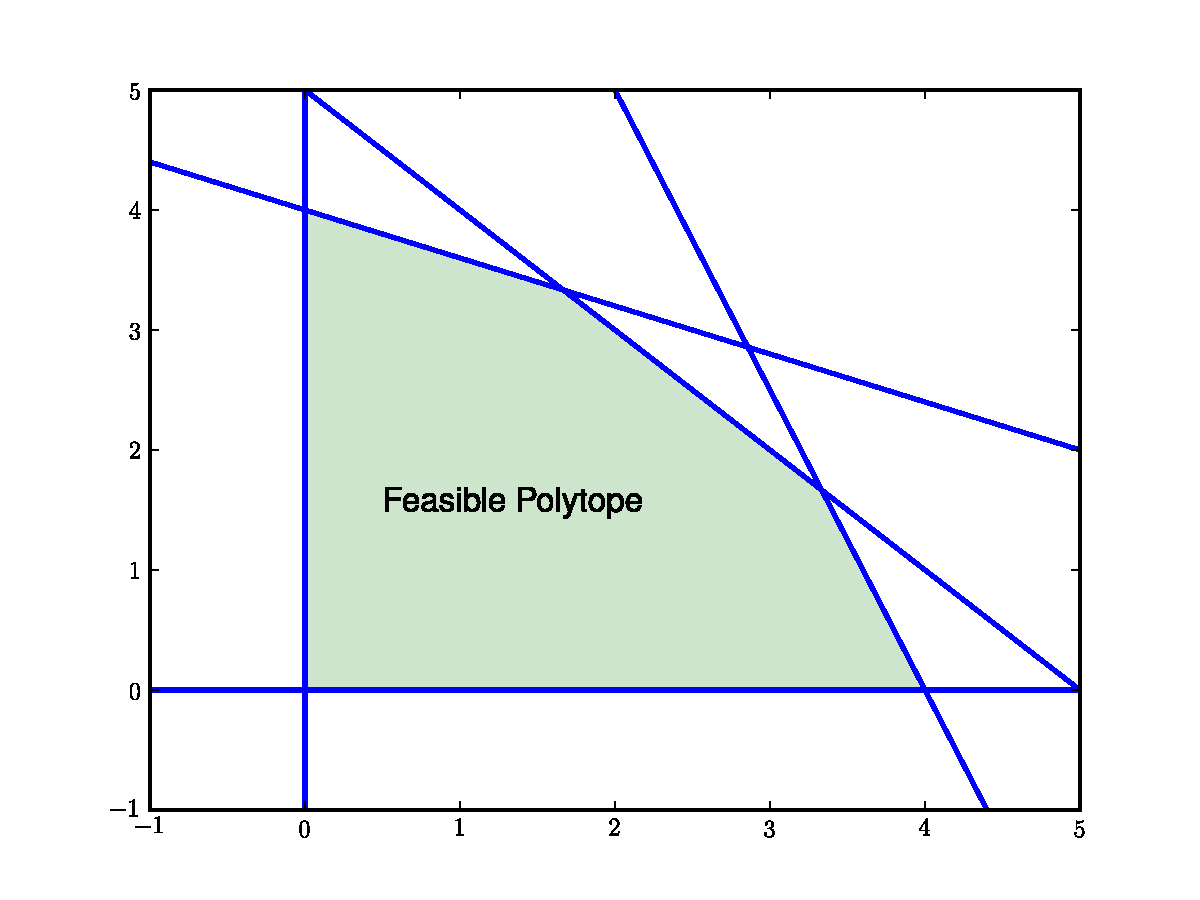
\includegraphics[width=\textwidth]{feasiblePolytope.pdf}
\caption{The feasible region for a linear program. The optimal point
is one of the vertices of the polytope.}
\label{fig:polytope}
\end{figure}

Implementing the Simplex Algorithm is straightforward, provided one carefully follows the procedure.
We will break the algorithm into several small steps, and write a function to perform each one.
To become familiar with the execution of the Simplex algorithm, it is helpful to work several examples by hand.

\section*{The Simplex Solver}
Our program will be more lengthy than many other lab exercises and will consist of a collection of functions working
together to produce a final result.
It is important to clearly define the task of each function and how all the functions will work together.
If this program is written haphazardly, it will be much longer and more difficult to read than it needs to be.
We will walk you through the steps of implementing the Simplex Algorithm as a Python class.
%Since the Simplex Algorithm assumes that all the variables are non-negative, we do not need any special logic for it.
%what is this previous statement saying? What 'special logic' would you need if the variables were negative?

For demonstration purposes, we will use the following linear program.
\begin{align*}
\text{maximize}\qquad & 3x_0 + 2x_1 \\
\text{subject to}\qquad
& x_0 - x_1 \leq 2 \\
& 3x_0 + x_1 \leq 5 \\
& 4x_0 + 3x_1 \leq 7 \\
& x_0, x_1 \geq 0.
\end{align*}

\subsection{Accepting a Linear Program}
Our first task is to determine if we can even use the Simplex algorithm.
Assuming that the problem is presented to us in standard form, we need
to check that the feasible region is nonempty.

\begin{problem}
Write a Python class that accepts a linear program and checks its feasibility.
You may implement the feasibility check directly into the class initialization method, or use a separate class method.
To simplify the implementation of your solver, we only check feasibility at the origin.
That is, check that $Ax \leq b$ when $x = 0$.
Return an error if the given program is infeasible at the origin.
Your class might have the following structure, where the linear program is accepted in the initialization method.
\begin{lstlisting}
class SimplexSolver(object):
    def __init__(self, c, A, b):
        if infeasible:
            print "Problem is infeasible"
\end{lstlisting}
\label{prob:initsolver}
\end{problem}
The inputs \li{c, A, b} are all NumPy arrays.
\subsection{Adding Slack Variables}
Our next step is to convert the inequality constraints $Ax \leq b$ into equality constraints
by introducing one slack variable for each constraint.
If the constraint matrix $A$ is an $m \times n$ matrix, then there are $m$ slack variables,
one for each row of $A$.
Grouping all of the slack variables into a vector of length $m$, denoted by $z$, our
constraints now take the form $Ax + z = b$.

When adding slack variables, it is useful represent all of your variables, both the original primal variables and
the additional slack variables, in a convenient manner.
One effective way is to refer to a variable by its subscript.
For example, we can use the integers $0$ through $n-1$ to refer to the original (non-slack) variables $x_0$ through
$x_{n-1}$, and we can use the integers $n$ through $n+m-1$ to track the slack variables (where the slack variable
corresponding to the $i$-th row of the constraint matrix is represented by the index $n+i-1$).

We also need some way to track which variables are basic and which variables are nonbasic.
A useful representation for the variables is a Python list (or NumPy array), where the elements of the list are integers.
Since we know how many basic variables we have ($m$, to be precise), we can partition the list so that all the basic
variables are kept in the first $m$ locations, and all the non-basic variables are stored at the end of the list.
The ordering of this list is important. In particular, if $i \leq m$, the $i$-th element of the list represents
the basic variable corresponding to the $i$-th row of $A$. Henceforth we will refer to this list as the \emph{index list}.

Initially, the basic variables are simply the slack variables.
In our example, we have 2 primal variables $x_0$ and $x_1$, and we must add 3 slack variables.
Thus, we instantiate the following index list:
\begin{lstlisting}
>>> L = [2, 3, 4, 0, 1]
\end{lstlisting}
Notice how the first $3$ entries of the index list are $2, 3, 4$, the indices representing the slack variables.
This reflects the fact that the basic variables at this point are exactly the slack variables.

As the Simplex Algorithm progresses, however, the basic variables change, and it will be necessary to swap
elements in our index list. Suppose the variable represented by the index $4$ becomes nonbasic, while
the variable represented by index $0$ becomes basic. We must swap these two entries in the index list.
This can be done in a single, efficient line of Python code:
\begin{lstlisting}
>>> L[2], L[3] = L[3], L[2]
>>> L
[2, 3, 0, 4, 1]
\end{lstlisting}
Now our index list tells us that the current basic variables have indices $2, 3, 0$.

\begin{problem}
Design and implement a way to store and track all of the basic and non-basic variables.

\emph{Hint: Using integers that represent the index of each variable is useful for Problem \ref{prob:blands}.}
\label{prob:slackvars}
\end{problem}

\subsection{Creating a Tableau}
After we have determined that our program is feasible, we need to create the \emph{tableau}, a construct
that tracks the state of the algorithm.
You may structure the tableau to suit your specific implementation.
Remember that your tableau will need to include in some way the slack variables that you created in Problem
\ref{prob:slackvars}.

There are many different ways to build your tableau.
One way is to mimic the tableau that is often used when performing the Simplex Algorithm by hand.
Define
\[
\bar{A} = \begin{bmatrix}
  A & I_m
\end{bmatrix},
\]
where $I_m$ is the $m \times m$ identity matrix,
and define
\[
\bar{c} = \begin{bmatrix}
  c\\
  0\\
  \vdots\\
  0
\end{bmatrix}.
\]
That is, $\bar{c} \in \mathbb{R}^{n+m}$ such that the first $n$ entries are $c$ and the final $m$ entries are zeros.
Then the initial tableau has the form
\begin{equation}
T = \begin{bmatrix}
    0 & -\bar{c}^T & 1  \\
    b & \bar{A} & 0
    \end{bmatrix}.
\label{eqn:hand_tab}
\end{equation}

The columns of the tableau correspond to each of the variables (both primal and slack), and the rows of the tableau
correspond to the basic variables. Using the convention introduced above
of representing the variables by indices in the index list, we have the following correspondence:
\[
\text{column } i \Leftrightarrow \text{index } i-2, \qquad i = 2, 3, \ldots, n+m+1,
\]
and
\[
\text{row } j \Leftrightarrow L_{j-1}, \qquad j = 2, 3, \ldots, m+1,
\]
where $L_{j-1}$ refers to the $(j-1)$-th entry of the index list.

For our example problem, the initial index list is
\[
L = (2, 3, 4, 0, 1),
\]
and the initial tableau is
\begin{equation*}
T = \begin{bmatrix}
    0 & -3 & -2 & 0 & 0 & 0 & 1\\
    2 & 1 & -1 & 1 & 0 & 0 & 0\\
    5 & 3 & 1 & 0 & 1 & 0 & 0\\
    7 & 4 & 3 & 0 & 0 & 1 & 0
    \end{bmatrix}.
\end{equation*}
The third column corresponds to index $1$, and the fourth row corresponds to index $4$, since this is the
third entry of the index list.

The advantage of using this kind of tableau is that it is easy to check the progress of your algorithm by hand.
The disadvantage is that pivot operations require careful bookkeeping to track the variables and constraints.

%I propose that we don't introduce the below tableau in the lab. It is less intuitive, and I think could lead to more confusion.
\begin{comment}
We can also use a tableau of the following format:
\begin{equation}
T = \begin{bmatrix}
    0 & c^T  & 0 \\
    0 & I_n & 0\\
    b & -A  & 0
\end{bmatrix}.
\label{eqn:matrix_tab}
\end{equation}
Here, $T$ is a square matrix of size $(n+m+1) \times (n+m+1)$.
The advantage of this form of the tableau is that all the pivot bookkeeping is built into the matrix.
For our example problem, the initial tableau of this form is
\begin{equation}
T = \begin{bmatrix}
        0 & 3 & 2 & 0 & 0 & 0 \\
        0 & 1 & 0 & 0 & 0 & 0 \\
        0 & 0 & 1 & 0 & 0 & 0 \\
        2 &-1 & 1 & 0 & 0 & 0 \\
        5 &-3 &-1 & 0 & 0 & 0 \\
        7 &-4 &-3 & 0 & 0 & 0
\end{bmatrix}.
\label{eqn:matrix_inittab}
\end{equation}
\end{comment}

\begin{problem}
Add a method to your Simplex solver that will create the initial tableau that you will use.
Using a NumPy array to represent your tableau will simplify several parts of the Simplex algorithm.
Your class may have the following structure at this point:
\begin{lstlisting}
class SimplexSolver(object):
    def __init__(self, c, A, b):
        if infeasible:
            print "LP is infeasible"

        self.makeTableau()

    def makeTableau(self):
        pass
\end{lstlisting}
\label{prob:maketableau}
\end{problem}

\subsection{Pivoting}
Pivoting is the mechanism that really makes Simplex useful.
Pivoting refers to the act of swapping basic and nonbasic variables, and transforming the tableau appropriately.
This has the effect of moving from one vertex of the feasible polytope to another vertex in a way that increases
the value of the objective function.
Depending on how you store your variables, you may need to modify a few different parts of your solver to reflect this swapping.

When initiating a pivot, you need to determine which variables will be swapped.
In the tableau representation, you first find a specific element on which to pivot, and the row and column that contain the pivot
element correspond to the variables that need to be swapped.
Row operations are then performed on the tableau so that the pivot column becomes an elementary vector.

Let's break it down, starting with pivot selection. We need to use some care when choosing the pivot element.
To find the pivot column, search from left to right along the top row of the tableau
(ignoring the first column), and stop once you encounter the first negative value. The index corresponding
to this column will be designated the \emph{entering index}, since after the full pivot operation, it will enter
the basis and become a basic variable.

Using our initial tableau $T$ in the example, we stop at the second column:
\[ T = \left[ \:
\begin{array}{*{7}{c}}
\cline{2-2}
0 & \multicolumn{1}{|c}{-3} & \multicolumn{1}{|c}{-2} & 0 & 0 & 0 & 1\\
2 & \multicolumn{1}{|c}{1} & \multicolumn{1}{|c}{-1} & 1 & 0 & 0 & 0\\
5 & \multicolumn{1}{|c}{3} & \multicolumn{1}{|c}{1} & 0 & 1 & 0 & 0\\
7 & \multicolumn{1}{|c}{4} & \multicolumn{1}{|c}{3} & 0 & 0 & 1 & 0\\
\cline{2-2}
\end{array}
\right] \]
We now know that our pivot element will be found in the second column. Our entering index is thus $0$.

Next, we select the pivot element from among the positive entries in the pivot column (ignoring the entry in the first row).
\emph{If all entries in the pivot column are non-positive, the problem is unbounded and has no solution.} In this case, the algorithm
should terminate.
Otherwise, assuming our pivot column is the $j$-th column of the tableau and that the positive entries of this column are
$T_{i_1, j}, T_{i_2, j}, \ldots, T_{i_k, j}$, we calculate the ratios
\[
\frac{T_{i_1,1}}{T_{i_1,j}}, \frac{T_{i_2,1}}{T_{i_2,j}}, \ldots, \frac{T_{i_k,1}}{T_{i_k,j}},
\]
and we choose our pivot element to be one that minimizes this ratio. If multiple entries minimize the ratio, then we utilize
\emph{Bland's Rule}, which instructs us to choose the entry in the row corresponding to the smallest index.
(Obeying this rule is important, as it prevents the possibility of the algorithm cycling back on itself infinitely.)
The index corresponding to the pivot row is designated as the \emph{leaving index}, since after the full pivot operation,
it will leave the basis and become a nonbasic variable.

In our example, we see that all entries in the pivot column (ignoring the entry in the first row, of course) are positive,
and hence they are all potential choices for the pivot element. We then calculate the ratios, and obtain
\[
\frac{2}{1} = 2,\quad \frac{5}{3} = 1.66...,\quad \frac{7}{4} = 1.75.
\]
We see that the entry in the third row minimizes these ratios. Hence, the element in the second column, third row is our designated
pivot element, and our leaving index is $L_2 = 3$:

\[ T = \left[ \:
\begin{array}{*{7}{c}}

0 & -3 & -2 & 0 & 0 & 0 & 1\\
2 & 1 & -1 & 1 & 0 & 0 & 0\\\cline{2-2}
5 & \multicolumn{1}{|c}{3} & \multicolumn{1}{|c}{1} & 0 & 1 & 0 & 0\\\cline{2-2}
7 & 4 & 3 & 0 & 0 & 1 & 0\\
\end{array}
\right] \]

\begin{comment}
If we are using the tableau representation in equation \ref{eqn:matrix_tab}, pivot operations are reduced to a simple matrix equation:
\[T = T + T_m \otimes T_n,\]
where $T_m$ is the column corresponding to the variable entering the basis and $T_n$ is a normalized vector corresponding to the variable leaving the basis.  The result of the equation is the new tableau.

For example, for the initial tableau, \ref{eqn:matrix_inittab}, we will demonstrate the first pivot operation.
We can do the entire pivot with a single outer product.
the first pivot should occur with $x_1$ leaving and $x_4$ entering.
In other words, we want to pivot at row $i = 4$ and column $j = 1$ in the tableau (the indices are offset by one because of the objective function and the row of constraints).

The row corresponding to $x_4$ is
\[
\begin{bmatrix} 5 &-3 &-1 & 0 & 0 & 0\end{bmatrix}.
\]
This represents the equation
\[
x_4 = 5 - 3x_1 - x_2.
\]
Our eventual goal is to solve for $x_1$ and substitute into the remaining rows of the tableau.
A simple method to accomplish this is to rewrite the equation so that we have zero on the left-hand side:
\[
0 = 5 - 3x_1 - x_2 - x_4.
\]
Now, we can normalize this equation so that the coefficient of $x_1$ is $-1$.
This is always accomplished by dividing the equation by the negative of the coefficient of $x_1$:
\begin{equation}
0 = \frac{5}{3} - x_1 - \frac{1}{3}x_2 - \frac{1}{3}x_4.
\label{eq:zero-equation}
\end{equation}
This is represented by the vector
\[
\begin{bmatrix} 5/3 & -1 & -1/3 & 0 & -1/3 & 0\end{bmatrix}.
\]
Since this left-hand side is zero, I can add any scalar multiple of this equation to any of the equations for $x_i$ and still have an equation for $x_i$.
For example, the equation for $x_5$ is
\[
x_5 = 7 - 4x_1 - 3x_2.
\]
Thus, I can add $-4$ times \eqref{eq:zero-equation} to this equation without changing the left-hand side:
\[ x_5 = 7 - 4x_1 - 3x_2 = 7 - 4x_1 - 3x_2 + -4\left(\frac{5}{3} - x_1 - \frac{1}{3}x_2 - \frac{1}{3}x_4\right) = \frac{1}{3} - \frac{5}{3}x_2 + \frac{4}{3} x_4.
\]
Notice that we end up with an equation that does not include $x_1$ and now has $x_4$, just like we wanted.
In fact, this works in all of our equations, including those for the objective function and even for $x_1$!
Since the coefficient of $x_1$ in \eqref{eq:zero-equation} is $-1$, when we scale it by the coefficient of $x_1$ in any particular row, the $x_1$ cancels out.
\[
T = T + \begin{bmatrix}3 \\ 1 \\ 0 \\ -1 \\ -3 \\ -4\end{bmatrix}\begin{bmatrix} 5/3 & -1 & -1/3 & 0 & -1/3 & 0\end{bmatrix}.
\]
The column vector is just the second column of $T$, which is the column containing the coefficients of $x_1$ in each row.
When we compute this sum, we obtain the tableau.
\[
T = \begin{bmatrix}
        5 &  0 & 1 & 0 & -1 & 0 \\
        5/3 & 0 &-1/3 & 0 &-1/3 & 0 \\
        0 & 0 & 1 & 0 & 0 & 0 \\
        1/3 & 0 & 4/3 & 0 & 1/3 & 0 \\
        0 & 0 & 0 & 0 & 1 & 0 \\
        1/3 & 0 & -5/3 & 0 & 4/3 & 0
\end{bmatrix}.
\]
\end{comment}
\begin{problem}
Write a method that will determine the pivot row and pivot column according to Bland's Rule.
\begin{comment}
\begin{definition}[Bland's Rule]
Choose the nonbasic variable with the smallest index that has a positive coefficient in the objective function
as the leaving variable.  Choose the basic variable with the smallest index among all the binding basic variables.
\end{definition}

Bland's Rule is important in avoiding cycles when performing pivots.
This rule guarantees that a feasible Simplex problem will terminate in a finite number of pivots.
\end{comment}
\label{prob:blands}
\end{problem}

The next step is to swap the entering and leaving indices in our index list.
In the example, we determined above that these indices are $0$ and $3$. We swap these two elements in our index list,
and the updated index list is now
\[
L = (2, 0, 4, 3, 1),
\]
so that the basic variables are given by the indices $2, 0, 4$.

Finally, we perform row operations on our tableau in the following way: divide the pivot row by the value of the pivot entry.
Then use the pivot row to zero out all entries in the pivot column above and below the pivot entry. In our example, we first divide
the pivot row by 3, and then zero out the two entries above the pivot element and the single entry below it:
\begin{align*}
\begin{bmatrix}
    0 & -3 & -2 & 0 & 0 & 0 & 1\\
    2 & 1 & -1 & 1 & 0 & 0 & 0\\
    5 & 3 & 1 & 0 & 1 & 0 & 0\\
    7 & 4 & 3 & 0 & 0 & 1 & 0
    \end{bmatrix} &\rightarrow
\begin{bmatrix}
    0 & -3 & -2 & 0 & 0 & 0 & 1\\
    2 & 1 & -1 & 1 & 0 & 0 & 0\\
    5/3 & 1 & 1/3 & 0 & 1/3 & 0 & 0\\
    7 & 4 & 3 & 0 & 0 & 1 & 0
    \end{bmatrix}\rightarrow\\
\begin{bmatrix}
    5 & 0 & -1 & 0 & 1 & 0 & 1\\
    2 & 1 & -1 & 1 & 0 & 0 & 0\\
    5/3 & 1 & 1/3 & 0 & 1/3 & 0 & 0\\
    7 & 4 & 3 & 0 & 0 & 1 & 0
    \end{bmatrix} &\rightarrow
\begin{bmatrix}
    5 & 0 & -1 & 0 & 1 & 0 & 1\\
    1/3 & 0 & -4/3 & 1 & -1/3 & 0 & 0\\
    5/3 & 1 & 1/3 & 0 & 1/3 & 0 & 0\\
    7 & 4 & 3 & 0 & 0 & 1 & 0
    \end{bmatrix}\rightarrow\\
\begin{bmatrix}
    5 & 0 & -1 & 0 & 1 & 0 & 1\\
    1/3 & 0 & -4/3 & 1 & -1/3 & 0 & 0\\
    5/3 & 1 & 1/3 & 0 & 1/3 & 0 & 0\\
    1/3 & 0 & 5/3 & 0 & -4/3 & 1 & 0
    \end{bmatrix}.
\end{align*}
The result of these row operations is our updated Tableau, and the pivot operation is complete.

\begin{problem}
Add methods to your Simplex solver that will perform a single pivot operation from start to completion.
You pivoting method should check for unboundedness.
If the problem is unbounded, return an exception to the user.
\end{problem}

\subsection{Termination and Reading the Tableau}
Up to this point, our algorithm accepts a linear program, adds slack variables, and creates the initial tableau. After
carrying out these initial steps, it then performs the pivoting operation iteratively until the optimal point is found.
How can we determine when the optimal point is found? The answer is to look at the top row of the tableau. More specifically,
before each pivoting operation, check whether all of the entries in the top row of the tableau (ignoring the entry in the first
column) are nonnegative. If this is the case, then we have already found an optimal solution, and so we terminate the algorithm.

The final step is to report the solution. The current state of the tableau and index list tells us everything we need to know.
The maximum value attained by the objective function is found in the upper leftmost entry of the tableau. The nonbasic variables,
whose indices are located in the last $n$ entries of the index list, all have the value $0$. The basic variables, whose indices
are located in the first $m$ entries of the index list, have values given by the first column of the tableau. Specifically, the basic
variable whose index is located at the $i$-th entry of the index list has the value $T_{i+1, 1}$.

In our example, suppose that our algorithm terminates with the tableau and index list in the following state:
\[
T = \begin{bmatrix}
5.2 & 0 & 0 & 0 & .2 & .6 & 1\\
.6 & 0 & 0 & 1 & -1.4 & .8 & 0\\
1.6 & 1 & 0 & 0 & .6 & -.2 & 0\\
.2 & 0 & 1 & 0 & -.8 & .6 & 0\\
\end{bmatrix}
\]
\[
L = (2, 0, 1, 3, 4).
\]
Then the maximum value of the objective function is $5.2$. The nonbasic variables have indices $3, 4$ and have the value $0$.
The basic variables have indices $2, 0,$ and $1$, and have values $.6, 1.6$, and $.2$, respectively.
In the notation of the original problem statement, the solution is given by
\begin{align*}
x_0 &= 1.6\\
x_1 &= .2.
\end{align*}

\begin{problem}
Write an additional method in your solver called \li{solve} that obtains the optimal solution and returns it in the format: \li{(maximum value, basic variables,
nonbasic variables)}, where the basic and nonbasic variables are represented as two dictionaries that map the index of the variable to
its corresponding value.

For example, in our example, we would return the tuple \li{(5.2, \{0: 1.6, 1: .2, 2: .6\}, \{3: 0, 4: 0\})}.
The correct format of this tuple is critical as this tuple of information will be used judge if your solver works!
\end{problem}

At this point, you should have a Simplex solver that is simple to use. The following code demonstrates how your solver is
expected to behave.

\begin{lstlisting}
>>> # initialize objective function and constraints
>>> c = np.array([3., 2])
>>> b = np.array([2., 5, 7])
>>> A = np.array([[1., -1], [3, 1], [4, 3]])

>>> # instantiate the simplex solver, then solve the problem
>>> solver = SimplexSolver(c, A, b)
>>> solver.solve()
(5.200,
 {0: 1.600, 1: 0.200, 2: 0.600},
 {3: 0, 4: 0})
\end{lstlisting}

If the linear program were infeasible at the origin or unbounded, we would expect the solver to alert the user by throwing an error.

Note that your simplex solver is not fully operational. It can't handle the case of infeasibility at the origin. This can be fixed by adding
methods to your class that solve the \emph{auxiliary problem} of finding an initial feasible tableau when the problem is not feasible at the
origin. Solving the auxiliary problem involves pivoting operations identical to those you have already implemented, so adding this functionality
should not be overly difficult.
\section*{The Product Mix Problem}
We now use our Simplex implementation to solve the \emph{product mix problem}, which in its basic form can be expressed as a simple linear program.
Suppose a manufacturer makes $n$ products using $m$ different resources (labor, raw materials, available machine time, etc).
The $i$-th product is sold at a unit price $p_i$, and there are at most $m_j$ units
of the $j$-th resource available. Additionally, each unit of the $i$-th product requires $a_{j,i}$ units of resource $j$.
Given that the demand for product $i$ is $d_i$ units in certain time period, how do we choose the optimal amount
of each product to manufacture in that time period, so as to maximize revenue while not exceeding the available resources?

Let  $x_1, x_2, \ldots, x_n$ denote the amount of each product to be manufactured.
The sale of product $i$ brings revenue in the amount of $p_ix_i$.
Then our objective function, the profit, is given by
\[
\sum_{i=1}^n p_ix_i.
\]
Additionally, the manufacture of product $i$ requires $a_{j,i}x_i$ units of resource $j$.
Thus, we have the resource constraints
\[
\sum_{i=1}^n a_{j,i}x_i \leq m_j
\]
for $j = 1, 2, \ldots, m$.
Finally, we have the demand constraints which tell us not to exceed the demand for the products:
\[
x_i \leq d_i
\]
for $i = 1, 2, \ldots, n$.
Certainly the variables $x_i$ are constrained to be nonnegative. We therefore have a linear program in the appropriate form that is feasible at the origin.
It is a simple task to solve the problem using our Simplex solver.

\begin{problem}
Solve the product mix problem for the data contained in the file \li{productMix.npz}. In this problem, there are 4 products and 3 resources.
The archive file, which you can load using the function
\li{np.load}, contains a dictionary of arrays. The array with key \li{'A'} gives the resource coefficients $a_{i,j}$ (i.e. the $(i,j)$-th entry
of the array give $a_{i,j}$). The array with key \li{'p'} gives the unit prices $p_i$. The array with key \li{'m'} gives the available resource
units $m_j$. The array with key \li{'d'} gives the demand constraints $d_i$.

Report the number of units that should be produced for each product.
\end{problem}
%---------------------------------------------------------------------------------------------------
%
%
% \section*{Auxiliary Problems}
%
% When one of the entries of $b$ is negative, we need to run an auxiliary problem to find a feasible point.
% Try adding $x_0$ as the last variable.
% That way you just need to add a single row and column to your current tableau $T$.
% You can check that subtracting $x_0$ from each of the constraints is the same as adding $x_0$ to each of the expressions for the slack variables.
% Since we also need write $x_0$ in terms of itself ($x_0 = x_0$), this is equivalent to setting the last column equal to 1 for all the rows corresponding to slack variables, plus one new row.
% We also need to change the objective function to $-x_0$.
% Let's let $N$ be the matrix for the auxiliary problem.
% Then we can construct it from $T$ using the code
% \begin{lstlisting}
% >>> N = zeros((s+1,s+1))
% >>> N[0:s,0:s] = T
% >>> N[n:s+1,s] = 1
% >>> N[0,s] = -1
% \end{lstlisting}
%
% Before you run simplex on this auxiliary tableau, make sure you do a pivot on the last column and the row corresponding to the smallest entry of $b$.
% Check that the objective function value is 0 when simplex finishes running.
% If not, your initial problem is infeasible.
% If the problem is feasible, get the system of equations from $N$ and put them back into $T$, leaving off the last row and column of $N$ (for $x_0$) and the first row (corresponding to the objective function).
% \begin{lstlisting}
% T[1:s,0:s] = N[1:s,0:s]
% \end{lstlisting}
% The last thing you need to do is insert your previous objective function.
% However, you need to re-write it in terms of the current nonbasic variables.
% Fortunately, $T$ currently contains all of your variables written in terms of the nonbasic variables.
% You can check (mathematically, or however you want to satisfy yourself) that
% \begin{lstlisting}
% T[0,0:s] = T[0,0:s]*T
% \end{lstlisting}
% will put the objective function into the first row, now written in terms of the new nonbasic variables.

\section*{Beyond Simplex}
The Computing in Science and Engineering journal listed Simplex as one of the top ten algorithms of the twentieth century.\cite{Nash2000}
Despite its popularity, like any other algorithm, Simplex has drawbacks.

In 1972, Victor Klee and George Minty Cube published a paper with several examples of worst-case polytopes for the Simplex algorithm.\cite{Klee1972}
In their paper, they give several examples of polytopes that the Simplex algorithm struggles to solve.

Consider the following linear program from Klee-Minty.
\begin{align*}
\text{max } & 2^{n-1}x_1 & + & 2^{n-2}x_2  & + & \cdots & + & 2x_{n-1} & + & x_n\\
\text{subject to } & x_1 &  &  &  &  &  &  &  &\leq 5\\
& 4x_1 & + & x_2 &  &  &  &  &  &\leq 25\\
& 8x_1 & + & 4x_2 & + & x_3 &  &  &  &\leq 125\\
& \vdots & &      &   &     &  &  &  &\vdots\\
& 2^n x_1 & + & 2^{n-1} x_2 & + & \cdots & + & 4x_{n-1} & + x_n &\leq 5\\
\end{align*}

% When $n = 3$, we have the initial tableau
% \begin*{equation*}
% \begin{bmatrix}
% 0 & 4 & 2 & 1 & 0 & 0 & 0\\
% 0 & 1 & 0 & 0 & 0 & 0 & 0\\
% 0 & 0 & 1 & 0 & 0 & 0 & 0\\
% 0 & 0 & 0 & 1 & 0 & 0 & 0\\
% 5 & -1 & 0 & 0 & 0 & 0 & 0\\
% 25 & -4 & -1 & 0 & 0 & 0 & 0\\
% 125 & -8 & -4 & -1 & 0 & 0 & 0\\
% \end{bmatrix}
% \end{equation*}
%
% After the first pivot with $x_1$ leaving and $s_1$ entering, we have the tableau
%
% \begin{equation*}
% \begin{bmatrix}
% 20 & 0 & 2 & 1 & -4 & 0 & 0\\
% 5 & 0 & 0 & 0 & -1 & 0 & 0\\
% 0 & 0 & 1 & 0 & 0 & 0 & 0\\
% 0 & 0 & 0 & 1 & 0 & 0 & 0\\
% 0 & 0 & 0 & 0 & 1 & 0 & 0\\
% 5 & 0 & -1 & 0 & 4 & 0 & 0\\
% 85 & 0 & -4 & -1 & 8 & 0 & 0\\
% \end{bmatrix}
% \end{equation*}
%
% \begin{problem}
% What is the final tableau for this Klee-Minty example with $n=3$?
% How many iterations does it take to arrive at the final tableau?
% \end{problem}
%
% \begin{problem}
% Using problem 1 as a guide, guess the optimum value of the Klee-Minty example with $n=20$.
% Then find the maximum value for the Klee-Minty example with $n=20$.
% How many iterations does it take to arrive at the final tableau?
% How long does the program take to run for only $20$ variables?
% \end{problem}

Klee and Minty show that for this example, the worst case has exponential time complexity.
With only $n$ constraints and $n$ variables, the simplex algorithm goes through $2^n$ iterations.
This is because there are $2^n$ extreme points and when starting at the point $x=0$, the simplex algorithm goes through all of the extreme points before reaching the optimal point $(0,0,\dots, 0, 5^n)$.
Other algorithms, such as interior point methods, solve this problem much faster because they are not constrained to follow the edges.


% \bibliography{./references}
